\section{Giới thiệu}
Mỗi trò chơi đều có bối cảnh ra đời, mục tiêu phát triển và phạm vi triển khai. Ngoài ra, không thể thiếu những điểm khác biệt so với các sản phẩm hiện có trên
thị trường. Trong phần này, nhóm sẽ làm rõ những điều trên.
\subsection{Bối cảnh và vấn đề đặt ra}
    Thị trường game hiện nay đang chứng kiến sự trỗi dậy mạnh mẽ của dòng game \textit{Social Deduction} (Suy luận xã hội) và \textit{Party Game}. Những cái tên như \textit{Among Us}, \textit{Goose Goose Duck} hay \textit{Party Animals} đã chứng minh một chân lý: người chơi hiện đại không chỉ tìm kiếm thử thách về kỹ năng, họ khao khát sự kết nối. Họ muốn một không gian ảo nơi họ có thể tương tác, lừa lọc, cười đùa và "tương tàn" với bạn bè mình.\\
    
    Bên cạnh đó, với công nghệ ngày càng phát triển ngày nay, các trò chơi điện tử từ đó cũng ngày càng được phổ biến với mọi người trên thế giới. Trong đó yếu tố 3D trong các trò chơi điện tử đã trở nên không quá xa lạ trên thế giới và ngày càng trở nên được yêu thích. Yếu tố 3D mang đến cho người chơi một gốc nhìn mới mẻ, rộng rãi và chân thực hơn, khả năng đem đến trải nghiệm tốt cho người chơi được cao hơn. Đồ họa 3D xuất hiện trong các trò chơi đã trở nên kích thích với không chỉ giới trẻ mà gần như với lứa tuổi trên thế giới.\\
    
    Tuy nhiên, khi nhìn vào các bản chuyển thể Board Game (trò chơi bàn cờ) lên nền tảng số hiện nay, nhóm nhận thấy một "lỗ hổng" rất lớn. Hầu hết các game Saboteur (Kẻ phá hoại) trên thị trường đều chỉ tập trung vào cơ chế bài bạc (2D) trên một mặt phẳng tĩnh. Điều này vô tình giết chết không khí của một buổi tụ tập. Cảm giác căng thẳng khi nhìn vào mắt đối phương, hay sự vui vẻ khi cùng nhau làm trò hề trong lúc chờ đến lượt đi... hoàn toàn biến mất.  \\
    
    Từ đó, nhóm đã chọn đề tài phát triển một trò chơi dạng Party Game kết hợp với board game và các hoạt động ngoài lề khác như thay đồ, đánh đàn, ... . Trò chơi kết hợp giữa board game, multiplayer và sự sáng tạo trong công nghệ trò chơi. Việc đưa các hoạt động ngoài lề vào trò chơi sẽ làm tăng thêm sự tương tác của các người chơi với nhau. Điều này có thể tạo nên sự mới lạ, thu hút người chơi khám phá các tính năng trong trò chơi, nhưng cũng cần bảo đảm giữ được các yếu tố cơ bản và tinh thần chiến thuật truyền thống của trò chơi chính là \textit{Saboteur} để giúp người chơi không bị quá xa lạ với trò chơi.

\subsection{Saboteur - Lựa chọn trong vô vàn board game}

Board game Saboteur ra mắt năm 2004, được thiết kế bởi Fréderic Moyersoen, nhanh chóng trở thành một trong những trò chơi nhóm nổi tiếng nhất nhờ lối chơi bluffing - tương tác - phản bội cực kỳ kịch tính. Lấy bối cảnh những người thợ mỏ cùng nhau đào đường hầm tìm kho báu nhưng luôn có kẻ phá hoại ẩn mình, Saboteur tạo nên sự pha trộn hoàn hảo giữa chiến thuật, đọc vị tâm lý và những màn phản đòn bất ngờ. Nhờ luật chơi đơn giản nhưng độ sâu chiến thuật cao, trò chơi phù hợp với nhiều độ tuổi và được dịch, phát hành rộng rãi trên toàn thế giới. Với tính chất tương tác mạnh và khả năng tạo ra vô số tình huống hài hước lẫn “plot twist”, Saboteur hoàn toàn xứng đáng được tái hiện trong một trò chơi online 3D nhiều người chơi, nơi người chơi không chỉ chơi bài mà còn giao tiếp, hành động và trải nghiệm cảm giác nghi kỵ - hợp tác sống động hơn bao giờ hết trong không gian cabin ảo.

\begin{figure}[H]
    \centering
    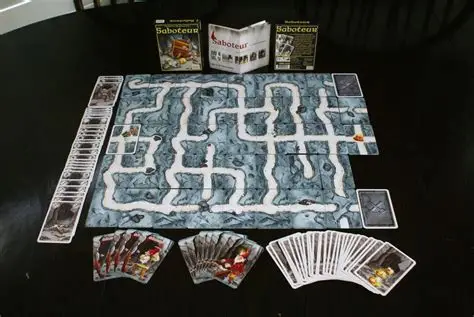
\includegraphics[width=0.75\linewidth]{5.Thiết kế//images/image.png}
    \caption{Bộ bài Saboteur đầy đủ}
    \label{fig:placeholder}
\end{figure}

Luật chơi của Saboteur \cite{saboteur2024} cụ thể như sau:

\begin{enumerate}
\item \textbf{Tổng quan và mục tiêu}

\begin{itemize}
  \item Số người chơi: 3--10.
  \item Mục tiêu:
  \begin{itemize}
      \item \textbf{Gold-Diggers}: mở đường từ Start đến Goal chứa vàng.
      \item \textbf{Saboteurs}: phá để Gold-Diggers không thể đến được vàng.
  \end{itemize}
\end{itemize}

\item \textbf{Trang bị trong bộ Saboteur}

\begin{itemize}
  \item 40 Thẻ đường (path cards): gồm 31 thẻ thông, 9 thẻ cụt
  \item 27 Thẻ hành động (action cards)
  \item 11 Thẻ vai trò (role cards)
\end{itemize}


\item \textbf{Bố trí bàn chơi (Setup)}

\begin{figure}[H]
    \centering
    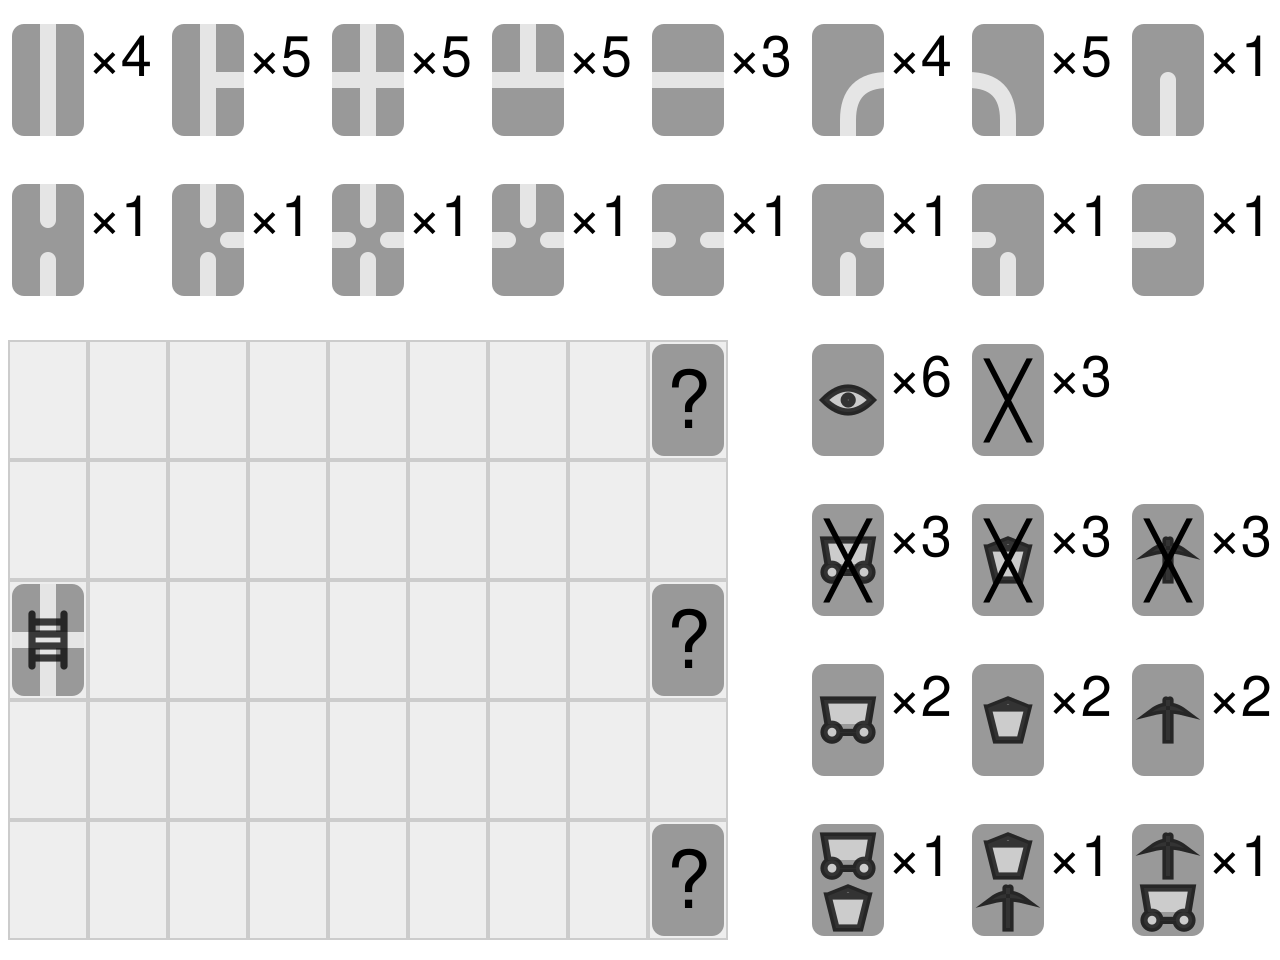
\includegraphics[width=0.75\linewidth]{5.Thiết kế//images/saboteurCards.png}
    \caption{Hình minh họa bộ thẻ và bàn chơi}
    \label{fig:cards-and-board}
\end{figure}


\begin{itemize}
  \item Đặt thẻ Start ở giữa bên trái.
  \item Đặt 3 thẻ Goal úp cách Start 7 khoảng thẻ: 1 giữa, 1 trên, 1 dưới.
  \item Vai trò và số thẻ phát cho mỗi người\\
  % \textbf{Số lượng vai trò theo số người chơi:}
    \begin{table}[h]
    \centering
        \begin{tabular}{|c|c|c|c|c|c|c|c|c|}
        \hline
        Tổng số Người chơi & 3 & 4 & 5 & 6 & 7 & 8 & 9 & 10 \\ \hline
        Số Saboteurs     & 1 & 1 & 2 & 2 & 3 & 3 & 3 & 4 \\ \hline
        Số Gold-Diggers  & 2 & 3 & 3 & 4 & 3 & 4 & 5 & 6 \\ \hline
        \end{tabular}
        \caption{Bảng số lượng vai trò theo số người chơi:}
        \label{tab:total-roles}
    \end{table}
    % \textbf{Số thẻ phát cho mỗi người:}
    \begin{table}[h]
    \centering
        \begin{tabular}{|c|c|c|c|c|c|c|c|c|}
        \hline
        Tổng số Người chơi      & 3 & 4 & 5 & 6 & 7 & 8 & 9 & 10 \\ \hline
        Thẻ mỗi người      & 6 & 6 & 6 & 5 & 5 & 4 & 4 & 4 \\ \hline
        \end{tabular}
        \caption{Bảng số thẻ phát cho mỗi người}
        \label{tab:cards-per-player}
    \end{table}

    \item Tất cả những lá bài còn lại được xáo lại thành chồng và để úp xuống bàn.
\end{itemize}


\item \textbf{Luật chơi}

\begin{itemize}
  \item Lượt xoay chiều kim đồng hồ.
  \item Mỗi lượt chọn một trong các hành động:
  \begin{enumerate}
    \item Đặt thẻ đường (path card).
    \item Chơi thẻ hành động (action card).
    \item Bỏ thẻ (discard).
  \end{enumerate}
  \item Sau khi xong lượt của mình, người chơi bốc lên thẻ trên cùng của deck, lượt chơi tiếp tục qua người tiếp theo.
  \item Gold-Diggers thắng khi có đường nối (phải là đường thông) từ start tới goal chứa vàng. Saboteurs thắng khi tất cả đã hết bài mà vẫn chưa nối được đường tới vàng.
\end{itemize}

% ========================================================
% 6. PATH CARDS
% ========================================================
\item \textbf{Thẻ đường (Path Cards)}
\begin{figure}[H]
    \centering
    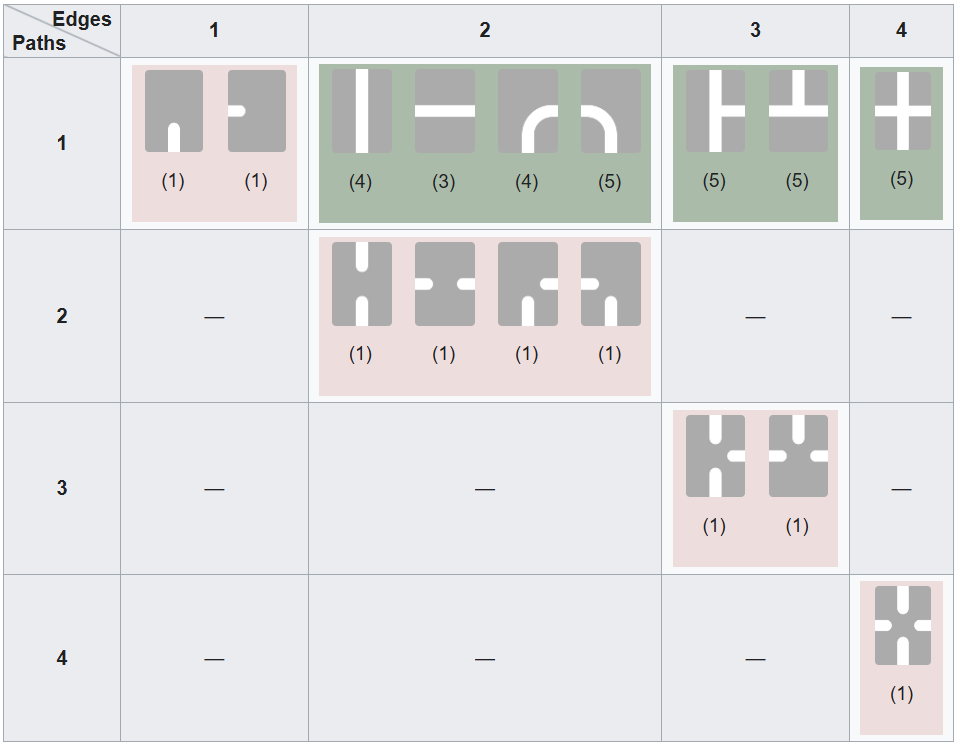
\includegraphics[width=0.75\linewidth]{5.Thiết kế//images/pathCards.png}
    \caption{Phân loại thẻ đường}
    \label{fig:placeholder}
\end{figure}
% \fbox{\parbox[c][4cm][c]{0.85\textwidth}{\centering (Placeholder) Các loại path cards}}
\begin{itemize}
  \item \textbf{Phân loại thẻ Đường}  
  Thẻ Đường (\emph{Path cards}) trong Saboteur được dùng để tạo ra mạng lưới đường hầm từ vị trí xuất phát đến các thẻ mục tiêu. Chúng được chia thành:
  \begin{itemize}
    \item \textbf{Thẻ đường thẳng}: nối liền hai đầu theo trục ngang hoặc dọc.
    \item \textbf{Thẻ giao nhau}: có nhiều nhánh rẽ, cho phép mở rộng đường theo nhiều hướng.
    \item \textbf{Thẻ cụt (dead-end)}: Có thể nối với các thể khác nhưng không được tính là thông đường.
    \item \textbf Các cạnh thẻ không có lối được tính là tường,  khiến người chơi không thể nối đường theo hướng đó.
  \end{itemize}

  \item \textbf{Cách đặt thẻ Đường hợp lệ}  
  Một thẻ Đường được xem là hợp lệ khi thỏa các điều kiện sau:
  \begin{itemize}
    \item Các đầu đường (lối ra) trên thẻ mới phải khớp với đầu đường của thẻ đã có trên bàn: đường nối với đường, tường nối với tường.
    \item Không được tạo ra một kết nối trái ngược (ví dụ: đầu đường mở nối vào tường bịt).
    \item Thẻ phải được đặt kề cạnh một thẻ đã có sẵn trong mạng lưới (không được “nhảy cóc”).
    % \item Người chơi không được phá vòng lặp đang tồn tại trừ khi dùng thẻ hành động chuyên biệt.
  \end{itemize}

  \item \textbf{Quy tắc xoay thẻ}  
  Tất cả thẻ Đường đều có thể được xoay 180° trước khi đặt xuống.  
  \begin{itemize}
    \item Người chơi không được xoay 90°; chỉ xoay 180° vì cấu trúc hầm được thiết kế theo hai hướng chính.
    \item Sau khi xoay, thẻ vẫn phải thỏa điều kiện kết nối hợp lệ như đã nêu ở mục trên.
  \end{itemize}

  \item \textbf{Phá đường bằng thẻ Bomb}  
  Thẻ \emph{Bomb} là thẻ hành động dùng để phá hủy một thẻ Đường đã được đặt trên bàn.
  \begin{itemize}
    \item Người chơi chọn một thẻ Đường bất kỳ (trừ thẻ Start và thẻ Goal) để loại bỏ.
    \item Sau khi phá, ô trống được để lại và không có thẻ nào tự động dịch chuyển vào.
    \item Bomb không được dùng để phá thẻ trên tay người chơi, chỉ phá thẻ đã đặt.
  \end{itemize}

\end{itemize}
% ========================================================
% 7. ACTION CARDS
% ========================================================
\item \textbf{Thẻ hành động (Action Cards)} 

Các thẻ hành động ảnh hưởng trực tiếp đến khả năng đặt thẻ đường hoặc quan sát thông tin trong ván chơi.  
Trong game có \textbf{3 loại công cụ}: 
\begin{itemize}
    \item Xe đẩy (\textit{Cart})
    \item Xẻng (\textit{Shovel})
    \item Mũ (\textit{Hat})
\end{itemize}

Nếu người chơi bị phá \textbf{bất kỳ một trong ba công cụ}, họ \textbf{không thể đặt thẻ đường}.  
Để sửa, người chơi phải dùng thẻ Repair tương ứng.

\begin{itemize}
    \item \textbf{Repair đơn}: sửa đúng 1 công cụ được chỉ định trên thẻ.
    \item \textbf{Repair kép}: sửa 1 trong 2 công cụ hiển thị trên thẻ (Có biến thể có thể sửa cả hai đồng thời).
\end{itemize}

\begin{table}[H]
\centering
\begin{tabular}{|c|p{7cm}|c|}
\hline
\textbf{Loại thẻ} & \textbf{Công dụng} & \textbf{Số lượng} \\ \hline
Sabotage & Phá 1 công cụ: Cart, Shovel hoặc Hat. Người bị phá không thể đặt Path cho đến khi được sửa. & 9 \\ \hline
Repair   & Sửa công cụ bị phá. Gồm: 6 thẻ đơn (mỗi loại công cụ 2 thẻ), 3 thẻ kép. & 9 \\ \hline
Map      & Cho phép xem lén 1 trong 3 thẻ Goal. Không được tiết lộ thông tin trừ khi tự nguyện. & 6 \\ \hline
Rockfall & Phá hủy 1 Path card trên bàn (trừ Start và 3 Goal). Thẻ bị phá được loại khỏi mỏ. & 3 \\ \hline
\end{tabular}
\end{table}

% \end{itemize}

\end{enumerate}
\subsection{Sáng tạo luật chơi mới - Biến thể Saboteur với  ngày đêm }
Biến thể mới giữ nguyên tinh thần bluffing và phản bội của Saboteur gốc nhưng bổ sung cơ chế pha \textbf{ngày} - \textbf{đêm}, thời gian giới hạn, tranh luận, bỏ phiếu và một số thẻ hành động mới mạnh mẽ hơn. Trò chơi vẫn chia hai phe: \textbf{Thiện (Gold-Diggers - Chó)} và \textbf{Ác (Saboteurs - Mèo)}, sử dụng bộ bài gồm thẻ đường (path cards) và thẻ hành động (action cards). Mục tiêu thắng thua giữ nguyên như phiên bản gốc.
\begin{enumerate}
\item \textbf{Chuẩn bị trước khi bắt đầu game}
\begin{itemize}
\item Chia vai trò (role cards) theo bảng phân bổ của phiên bản gốc (xem bảng \ref{tab:total-roles} - số lượng Saboteurs và Gold-Diggers theo tổng số người chơi).
\item \textbf{Thêm số lượng thẻ đường}: Sử dụng toàn bộ thẻ đường của bộ gốc, nhưng \textbf{ngẫu nhiên loại bỏ 10 thẻ đường} trước khi xào bài và để không ai biết chính xác số lượng cũng như loại thẻ đường nào còn lại trong bộ bài.
\item Chia bài cho mỗi người chơi như cũ theo bảng \ref{tab:cards-per-player} 
\item Xào phần bài còn lại thành chồng bài úp (draw pile).
\item Bố trí bàn chơi giống phiên bản gốc (xem hình \ref{fig:cards-and-board}).
\end{itemize}
\item \textbf{Cấu trúc một round}
\\
Mỗi round được chia thành hai pha chính: \textbf{Đêm} và \textbf{Ngày}.
\\
\textbf{Đêm (Night Phase):}
\begin{itemize}
\item Màn hình/bản đồ tối lại, người chơi \textbf{không nhìn thấy bất kỳ thay đổi nào trên bản đồ} ngoại trừ thông tin lượt hiện tại.
\item Thứ tự lượt chơi trong đêm được \textbf{xếp ngẫu nhiên} (không theo chiều kim đồng hồ như bản gốc).
\item Mỗi người chơi lần lượt thực hiện lượt:
\begin{itemize}
\item Bản đồ tạm thời hiện ra cho riêng người đó.
\item Trong \textbf{15--30 giây} (có thể tùy chỉnh), người chơi thực hiện một trong các hành động quen thuộc:
\begin{enumerate}
\item Đặt thẻ đường (path card) – phải tuân thủ đầy đủ quy tắc kết nối và xoay thẻ như bản gốc.
\item Chơi thẻ hành động (action card).
\item Bỏ bài (discard).
\end{enumerate}
\item Sau khi hết thời gian hoặc xác nhận hành động, bản đồ lại tối đi với người chơi đó.
\item Bốc 1 lá bài từ chồng bài úp (nếu còn).
\end{itemize}
\item Khi tất cả người chơi đã hoàn thành lượt trong đêm, pha Đêm kết thúc và chuyển sang pha Ngày.
\end{itemize}



\textbf{Ngày (Day Phase):}
\begin{itemize}
\item Bản đồ được chiếu sáng hoàn toàn, mọi người chơi cùng nhìn thấy toàn bộ thay đổi đã xảy ra trong pha Đêm.
\item Người chơi có \textbf{60 giây} (có thể tùy chỉnh) để \textbf{trò chuyện, tranh luận, biện minh} và đọc vị nhau.
\item Cuối pha Ngày, thực hiện \textbf{bỏ phiếu}:
\begin{itemize}
\item Có thể vote \textbf{skip} (không loại ai) hoặc vote một người chơi cụ thể.
\item Người bị vote nhiều phiếu nhất sẽ bị \textbf{cấm chơi 1 round tiếp theo} (không được hành động trong pha Đêm của round sau).
\end{itemize}
\end{itemize}

\item \textbf{Kết thúc game}
Giữ nguyên luật thắng thua của phiên bản gốc:
\begin{itemize}
\item Phe Thiện (Chó) thắng nếu có đường thông hợp lệ từ thẻ Start đến thẻ Goal chứa vàng.
\item Phe Ác (Mèo) thắng nếu hết bài trên tay tất cả người chơi mà vẫn chưa nối được đường đến vàng.
\end{itemize}
\item \textbf{Thẻ hành động mới (bổ sung thêm vào bộ bài)}
\begin{table}[H]
\centering
\begin{tabular}{|l|p{7cm}|p{5cm}|}
\hline
\textbf{Tên thẻ} & \textbf{Công dụng} & \textbf{Ghi chú} \\ \hline
Shield & Người chơi sẽ có khiên vĩnh viễn có thể đỡ được 1 đòn tấn công phá công cụ (Cart, Shovel, Hat) bởi thẻ Sabotage. & Có thể áp dụng cho bất cứ ai, không tích lũy \\ \hline
Binoculars & Khi sử dụng thẻ này, người chơi được nhìn thấy toàn bộ bản đồ từ lúc chơi thẻ cho đến hết Đêm hiện tại. & Có thể áp dụng cho bất cứ ai\\ \hline
Swap Goals & Trong Đêm, tráo vị trí ngẫu nhiên hoặc chỉ định của 3 thẻ Goal (khi chúng vẫn đang úp). & Thay đổi vị trí kho vàng thực sự \\ \hline
\end{tabular}
\caption{Các thẻ hành động mới}
\end{table}
\end{enumerate}


\subsection{Mục tiêu của đề tài}
    Từ những phân tích về thực trạng và nhu cầu thị trường nêu trên, nhóm thực hiện đề tài xác định các mục tiêu cốt lõi cần đạt được như sau:\\

    \textbf{Thứ nhất, số hóa và tự động hóa trọn vẹn luật chơi Saboteur:}
    Mục tiêu đầu tiên là xây dựng một hệ thống logic game hoàn chỉnh, đảm bảo tuân thủ chính xác luật chơi gốc của board game Saboteur. Hệ thống phải tự động xử lý các thao tác phức tạp như chia bài, kiểm tra vai trò (Role), thuật toán loang để xác định đường đi liên thông từ điểm xuất phát đến kho báu, và tính toán thắng thua. Điều này nhằm loại bỏ sự rườm rà trong việc thiết lập bàn chơi (setup) thủ công, giúp người chơi tập trung hoàn toàn vào chiến thuật.\\
    
    \textbf{Thứ hai, xây dựng thêm phiên bản Saboteur mở rộng kết hợp cơ chế Ma Sói (Werewolf):} Mục tiêu của đề tài là phát triển thêm một phiên bản Saboteur hoàn toàn mới bằng cách tích hợp các yếu tố đặc trưng của Ma Sói nhằm tăng tính chiến thuật và tương tác giữa người chơi. Cụ thể, trò chơi được thiết kế với hai giai đoạn ngày và đêm, cho phép người chơi thảo luận, suy luận và bỏ phiếu trong pha ngày để xác định người bị nghi ngờ; người có số phiếu cao nhất sẽ bị cấm lượt đi trong đêm tiếp theo. Sự kết hợp giữa cơ chế xây dựng đường đi của Saboteur và yếu tố ẩn vai trò, đấu trí của Ma Sói giúp tạo ra trải nghiệm chơi mới mẻ, kịch tính và giàu tính chiến thuật hơn so với các phiên bản hiện có.\\
    
    \textbf{Thứ ba, xây dựng môi trường tương tác xã hội 3D:}
    Khác với các ứng dụng chơi bài 2D truyền thống, mục tiêu của nhóm là tạo ra một không gian 3D sống động – nơi người chơi không chỉ là những cái tên trên bảng điểm. Người chơi sẽ được hóa thân vào các nhân vật (Avatar), có khả năng di chuyển tự do trong không gian sảnh chờ (Lobby) và bàn chơi. Mục tiêu là tái hiện cảm giác "tụ tập" thực tế, nơi các tương tác vật lý và phi ngôn ngữ được đề cao.\\
    
    \textbf{Thứ tư, phát triển các tính năng giải trí bổ trợ:}
    Để giải quyết bài toán "thời gian chết" (downtime) khi chờ đợi người khác đánh bài hoặc chờ đủ người tạo phòng, nhóm đặt mục tiêu tích hợp các mini-features mang tính giải trí cao. Cụ thể là hệ thống nhạc cụ ảo (cho phép người chơi tương tác phím để tạo âm thanh) và hệ thống thời trang (thay đổi ngoại hình nhân vật). Đây là yếu tố then chốt để giữ chân người chơi và tạo nên sự vui nhộn đặc trưng của dòng Party Game.\\
    
    \textbf{Thứ năm, hoàn thiện kỹ thuật Multiplayer thời gian thực:}
    Ứng dụng kiến thức về lập trình mạng để xây dựng hệ thống Client-Host ổn định. Đảm bảo sự đồng bộ mượt mà về vị trí nhân vật, trạng thái bàn chơi và các tương tác thời gian thực giữa nhiều người chơi khác nhau, giảm thiểu độ trễ (latency) để trải nghiệm không bị gián đoạn.
    
\subsection{Phạm vi thực hiện}

    Về nền tảng, trò chơi hướng đến việc chơi trò chơi trên nền tảng Window từ phiên bản Window 7 trở lên.
    
    Về đối tượng hướng đến của trò chơi, trò chơi hướng đến tất cả mọi người ở mọi lứa tuổi cần sự giải trí, sự mới mẻ, sự cạnh tranh và tư duy giải đố.


\subsection{Ý nghĩa và tính ứng dụng của đề tài}

    \textbf{Ý nghĩa khoa học và thực tiễn:}
    Việc thực hiện đề tài "Fishy Business" không chỉ là việc tạo ra một sản phẩm giải trí đơn thuần, mà còn là cơ hội để nhóm áp dụng tổng hợp các kiến thức nền tảng của ngành Khoa học máy tính.
    \begin{itemize}
        \item \textit{Thử thách về Lập trình mạng:} Đồng bộ hóa trạng thái trong môi trường 3D là một bài toán khó, đòi hỏi sự hiểu biết sâu sắc về cấu trúc gói tin, băng thông và xử lý độ trễ.
        \item \textit{Tư duy Thiết kế hệ thống (System Design):} Việc kết hợp giữa logic chặt chẽ của một game bài (Turn-based) với sự tự do của một game nhập vai (Real-time 3D) đòi hỏi một kiến trúc phần mềm linh hoạt, dễ bảo trì và mở rộng (Design Patterns).
    \end{itemize}
    
    \textbf{Tính ứng dụng:}
    \begin{itemize}
        \item \textit{Giải trí và Kết nối:} Trong bối cảnh làm việc và học tập từ xa ngày càng phổ biến, sản phẩm đóng vai trò là cầu nối giúp bạn bè, đồng nghiệp có không gian để "gặp gỡ" và giải trí cùng nhau mà không bị giới hạn bởi khoảng cách địa lý.
        \item \textit{Tiềm năng mở rộng:} Dự án được xây dựng với kiến trúc hướng đối tượng (OOP), do đó có thể dễ dàng mở rộng để tích hợp thêm nhiều board game khác nhau (như Ma Sói, Mèo Nổ) vào cùng một game trong tương lai, hướng tới mô hình "Metaverse" thu nhỏ cho board game.
    \end{itemize}

\subsection{So sánh một số game tương tự trên thị trường}
Để định vị sản phẩm rõ ràng hơn, nhóm tiến hành so sánh \textit{Fishy Business} với các sản phẩm cạnh tranh trên nền tảng PC và Web.

\subsubsection{Tabletop Simulator (PC - Steam)}
Đây là "tượng đài" của dòng game mô phỏng board game trên PC.
\begin{itemize}
    \item \textbf{Điểm mạnh:} Mô phỏng vật lý cực kỳ chân thực, kho game khổng lồ từ Workshop.
    \item \textbf{Điểm yếu cần khắc phục:} Tabletop Simulator là một môi trường "Sandbox" thuần túy. Nó không có luật chơi tự động (người chơi phải tự tính điểm, tự xào bài bằng tay ảo). Hơn nữa, nó khá nặng nề và phức tạp cho những người chơi casual (phổ thông). Người chơi không có nhân vật để đi lại tương tác với môi trường, dẫn đến thiếu cảm giác kết nối xã hội.
\end{itemize}

\subsubsection{Board Game Arena (Web-based)}
Nền tảng chơi board game trên trình duyệt web rất phổ biến.
\begin{itemize}
    \item \textbf{Điểm mạnh:} Nhanh, tiện, chạy trên mọi trình duyệt, luật chơi tự động hóa tốt.
    \item \textbf{Điểm yếu cần khắc phục:} Đồ họa 2D hoàn toàn tĩnh. Trải nghiệm chơi giống như đang làm việc với một file Excel có hình ảnh hơn là chơi game. Không có âm nhạc, không có không khí, không có tương tác giữa các người chơi ngoài khung chat text bé tí.
\end{itemize}

\subsubsection{Sự khác biệt của Fishy Business}
\textit{Fishy Business} chọn một lối đi riêng trên PC:
\begin{itemize}
    \item \textbf{Trải nghiệm 3D Native:} Không phải là web game, đây là một ứng dụng Windows Standalone tận dụng sức mạnh đồ họa để tạo ra không gian đẹp mắt.
    \item \textbf{Kết hợp hoàn hảo:} Nhóm lấy sự tiện lợi (luật chơi tự động) của \textit{Board Game Arena} kết hợp với sự tự do, vui nhộn (di chuyển, nghịch ngợm) của các game như \textit{Overcooked} hay \textit{Party Animals}.
    \item \textbf{Tính năng độc nhất:} \textit{Fishy Business} kết hợp cơ chế xây dựng đường đi của Saboteur với yếu tố ẩn vai trò và suy luận theo phong cách Ma Sói trong hai pha ngày – đêm, kèm hệ thống thảo luận và bỏ phiếu. Đặc biệt, cơ chế “cấm lượt đi” tạo ra biến động chiến thuật liên tục, mang lại trải nghiệm mới lạ và kịch tính hơn so với Saboteur truyền thống.
\end{itemize}

\newpage